\documentclass[11pt]{article}
\usepackage[T1]{fontenc}
\usepackage[utf8]{inputenc}
\usepackage[a4paper,margin=2.3cm]{geometry}
\usepackage{amsmath,amssymb,amsthm}
\usepackage{booktabs,enumitem,graphicx}
\usepackage{tikz}\usetikzlibrary{arrows.meta,positioning,fit,backgrounds}
\usepackage[hidelinks]{hyperref}
\setlength{\emergencystretch}{2.5em}\hbadness=2500
\usepackage{xcolor}

\newcommand{\preuve}{{\small\textbf{[preuve]}}}
\newcommand{\num}{{\small\textbf{[num\'erique]}}}
\newcommand{\conj}{{\small\textbf{[conjecture]}}}
\newcommand{\heur}{{\small\textbf{[heuristique]}}}
\newcommand{\spec}{{\small\textbf{[sp\'eculation]}}}
\newcommand{\ouv}{{\small\textbf{[ouvert]}}}
\newcommand{\Spole}{\mathrm{S}}
\newcommand{\Npole}{\mathrm{N}}
\newcommand{\Mp}{M_{\mathrm{Pl}}}
\newcommand{\lP}{\ell_P}
\newcommand{\Stwo}{S^2_{\text{\'ech}}}
\definecolor{inp}{HTML}{1F4E79}\definecolor{sec}{HTML}{2E7D32}\definecolor{lnk}{HTML}{B23A2E}

\theoremstyle{definition}
\newtheorem{post}{Postulat}
\newtheorem{defi}{D\'efinition}

\title{\textbf{Unit\'e 5 --- Compactification sph\'erique de l'espace d'\'echelle}\\[2mm]
\large La latitude comme coordonn\'ee de renormalisation dirig\'ee~: le verrou $\infty^\ast$ lev\'e,
au prix de l'enroulement et de la dualit\'e\\[1mm]
\normalsize\textit{version int\'egr\'ee de travail --- corps $+$ Annexes A (singularit\'e/cl\^oture),
B (gel d'horloge), C (carte d'embo\^itement), D (test cosmologique), E (sonde de c\oe ur)}}
\author{Hassane Bakkaoui\\\small Chercheur ind\'ependant --- \texttt{bakkahassa@hotmail.com}}
\date{\small juin 2026 \;\textbullet\; document autonome --- calculs reproductibles (hep-th / gr-qc / quant-ph)}

\begin{document}
\maketitle

\begin{abstract}
\noindent Ce travail part d'une conviction et d'une seule hypoth\`ese. La conviction~: l'\'echelle \`a
laquelle on regarde l'univers --- du grain de Planck \`a l'horizon cosmologique --- n'est peut-\^etre pas
un simple param\`etre ext\'erieur, mais une g\'eom\'etrie \`a part enti\`ere. L'hypoth\`ese~: faire de
cette \'echelle une dimension interne compacte, \'ecrire la seule action qu'elle autorise, et laisser
tomber les cons\'equences. Rien n'est import\'e d'un mod\`ele existant~; on pose la g\'eom\'etrie, et on
regarde ce qu'elle dit.

\smallskip
\noindent Le programme ant\'erieur enroulait l'\'echelle en un tore, collant le plus petit et le plus grand
en un point unique. Cette Unit\'e fait un seul geste~: s\'eparer ce point en \emph{deux p\^oles distincts}
--- Planck d'un c\^ot\'e, l'infini de l'autre --- ce qui porte l'objet compact \`a une \emph{sph\`ere}. Ce
geste, \`a lui seul, lib\`ere une tension que le cercle imposait~: une fl\`eche d'\'echelle dirig\'ee
redevient possible, au prix de l'enroulement et de la dualit\'e d'inversion.

\smallskip
\noindent Ce qui distingue alors ce cadre n'a pas \'et\'e ajout\'e~: c'est \emph{tomb\'e de la structure}.
Une coordonn\'ee de renormalisation qui se trouve \^etre, du m\^eme coup, une fonction monotone de la
g\'eom\'etrie. Une horloge quantique et une fluctuation gravitationnelle qui se r\'ev\`elent \^etre les
deux vibrations d'un m\^eme oscillateur --- \'egales au repos, l\'eg\`erement d\'ecal\'ees d\`es qu'on les
agite. Une poign\'ee de nombres, fix\'es une seule fois par le rayonnement micro-onde, et qui doivent
ensuite gouverner six secteurs \`a la fois --- et qui y parviennent. Ces traits ne sont emprunt\'es \`a
personne~; ils sont la signature interne d'une seule id\'ee pouss\'ee jusqu'au bout. C'est l\`a, et non
dans une pi\`ece rapport\'ee, que le cadre diff\`ere des autres.

\smallskip
\noindent Nous disons aussi, sans d\'etour, ce que le cadre ne donne pas. Mis \`a l'\'epreuve de
l'observation, sa seconde dimension reste muette~: l'horloge, parce qu'elle est universelle, ne laisse pas
d'empreinte propre dans le spectre primordial, et le c\oe ur o\`u elle agirait vraiment est noy\'e sous une
courbure inaccessible. Ce qui est mesurable aujourd'hui ne le s\'epare pas encore de l'inflation ordinaire.
Nous avons pr\'ef\'er\'e tracer cette fronti\`ere nettement plut\^ot que de l'entretenir dans le flou.

\smallskip
\noindent Ce n'est donc ni une unification, ni une promesse d'observation. C'est une \emph{architecture}
--- coh\'erente, sur-d\'etermin\'ee, et enti\`erement issue d'elle-m\^eme --- propos\'ee comme une
fa\c{c}on de penser ensemble l'\'echelle, la gravitation et le temps quantique. Chaque \'enonc\'e du texte
porte son statut.

\smallskip
\noindent\textbf{Statuts}~: \preuve\ exact~; \num\ reproductible~; \conj\ argument\'e~;
\heur\ analogie~; \spec\ sp\'eculatif~; \ouv\ \`a \'etablir. \emph{Aucune conjecture n'est pr\'esent\'ee
comme un th\'eor\`eme.}
\end{abstract}

\section{Reformulation synth\'etique de l'intuition}
Le programme ant\'erieur (Unit\'es~1--4) repose sur une hypoth\`ese g\'eom\'etrique unique~: les axes
log-\'echelle sont des cercles internes. Projection st\'er\'eographique
$\psi=2\arctan[\ln(\lambda/\lP)]$ (axe spatial, face gravitationnelle) et
$\chi=2\arctan[\ln(\tau/\tau_P)]$ (axe temporel, face quantique/horloge HDEQ), p\^oles $\pm\pi$
identifi\'es en $\infty^\ast$, origine $\psi=\chi=0$ le point de Planck~$P$. Deux cercles $\to$ tore
$T^2=S^1_\psi\times S^1_\chi$.

Le verrou $\infty^\ast$~: sur un cercle, aucune fonction continue, univalu\'ee, strictement monotone
n'existe. L'identification UV$\equiv$IR est ainsi \emph{en m\^eme temps} source de l'enroulement et
obstruction \`a un flot d'\'echelle dirig\'e. Le tore poss\`ede la dualit\'e et l'enroulement \emph{ou} un
flot RG dirig\'e, jamais les deux.

\textbf{La modification.} On d\'enoue l'identification en \emph{deux p\^oles distincts}~: P\^ole Sud
$\Spole=$ Planck ($\lP$), P\^ole Nord $\Npole=$ infiniment grand. L'objet compact devient $\Stwo$~:
\begin{itemize}[nosep]
\item \emph{latitude} ($\theta$, ou $\cos\theta$)~: coordonn\'ee d'\'echelle \emph{dirig\'ee},
Planck~$\to$~infini, Morse \`a deux points critiques (les p\^oles)~; face gravitationnelle/cosmologique~;
\item \emph{azimut} ($\varphi$, p\'eriodique)~: phase / horloge interne, h\'eritier du cercle temporel
$\chi$~; face quantique.
\end{itemize}
En s\'eparant la boucle (azimut) de la direction (latitude), la sph\`ere \'echappe au verrou. Prix
topologique~: $\pi_1(\Stwo)=0$ d\'etruit l'enroulement, $\pi_2(\Stwo)=\mathbb{Z}$ fait migrer la charge.

\section{D\'efinitions et notations unifi\'ees}
\begin{post}[ar\`ene]\label{P1}
$\mathcal{M}=\mathcal{M}^{3+1}\times\Stwo$, $\Stwo$ cible interne ($\sigma$-mod\`ele). Champ
$n:\mathcal{M}^{3+1}\to\Stwo$, $n=(\sin\theta\cos\varphi,\sin\theta\sin\varphi,\cos\theta)$, $|n|=1$,
$\theta\in[0,\pi]$, $\varphi\in[0,2\pi)$.
\end{post}
\begin{post}[assignation des \'echelles]\label{P2}
Latitude $=$ \'echelle spatiale dirig\'ee, $\theta=2\arctan[\ln(\lambda/\lP)]$, $\lambda\ge\lP$~:
$\Spole:\theta{=}0\Leftrightarrow\lambda{=}\lP$, $\Npole:\theta{=}\pi\Leftrightarrow\lambda{\to}\infty$.
Azimut $=$ phase de l'\'echelle temporelle (r\^ole d'horloge HDEQ), p\'eriodique. Lecture alternative
st\'er\'eographique (latitude $=$ module conjoint, azimut $=$ rapport) cit\'ee au \S\ref{sec:pertes}.
\end{post}
\begin{post}[m\'etrique-cible, couplage, potentiel]\label{P3}
$G_{\text{cible}}=\omega(d\theta^2+\sin^2\!\theta\,d\varphi^2)$, $\omega=f_s^2>0$. D\'ependance en
latitude seule (pour pr\'eserver l'isom\'etrie azimutale $U(1)$)~:
\begin{equation}\label{eq:fV}
f(\theta)=1+\beta\cos\theta,\qquad V(\theta)=\alpha(1-\cos\theta),\qquad |\beta|<\tfrac12,\ \alpha>0.
\end{equation}
\end{post}
\begin{defi}[action, rep\`ere de Jordan]
\begin{equation}\label{eq:action}
S=\int d^4x\sqrt{-g}\Big[\tfrac12 fR-\tfrac12\omega(\partial\theta)^2
-\tfrac12\omega\sin^2\!\theta\,(\partial\varphi)^2-V\Big],\quad \Mp=\hbar=c=1.
\end{equation}
\end{defi}
\noindent P\^oles~: $f(\Spole)=1+\beta$, $V(\Spole)=0$ ($\Lambda=0$, vrai vide)~;
$f(\Npole)=1-\beta$, $V(\Npole)=2\alpha$ (faux vide dS). Le terme azimutal s'annule aux p\^oles.
\begin{defi}[charge $\pi_2$]
$Q_2=\frac{1}{4\pi}\int_\Sigma n\cdot(\partial_a n\times\partial_b n)\,dS^{ab}\in\mathbb{Z}$
(degr\'e de $n|_\Sigma:\Sigma\cong S^2\to\Stwo$). Remplace l'enroulement.
\end{defi}
\begin{defi}[r\'eduction m\'eridienne]\label{def:merid}
Sur $\varphi=\mathrm{const}$, l'action \eqref{eq:action} devient l'action mono-axe de l'Unit\'e~2
($\psi\mapsto\theta$)~: m\^emes EOM, m\^eme rep\`ere d'Einstein ($\tilde g=fg$, $U=V/f^2$,
$K=\omega/f+\tfrac32(f'/f)^2$). \preuve\ \emph{La diff\'erence sph\`ere/cercle est globale, non locale.}
\end{defi}

\section{Structure math\'ematique centrale}
\preuve\ $\pi_1(\Stwo)=0$, $\pi_2(\Stwo)=\mathbb{Z}$~: les kinks et l'enroulement $N=\tfrac12,1$
disparaissent~; une charge enti\`ere Skyrmion/monop\^ole appara\^it. La charge migre $\pi_1\to\pi_2$.

\preuve\ $\cos\theta$ est Morse, univalu\'ee, $d(\cos\theta)=-\sin\theta\,d\theta$ s'annulant aux seuls
p\^oles~: strictement monotone le long de tout m\'eridien --- l'antith\`ese de l'obstruction du verrou.

\preuve\ Isom\'etrie azimutale $U(1)$ ($\varphi\to\varphi+c$), courant
$J^\mu=\omega\sin^2\!\theta\,\partial^\mu\varphi$. Aux p\^oles $\sin^2\!\theta\to0$~: $U(1)$ trivial,
\emph{aucun Goldstone} si le vide est polaire.

\section{R\'esultats des deux KILL-TESTS (sans complaisance)}

\subsection{KILL-TEST 1 --- la c-fonction dynamique}
\textbf{(a) Permission.} \preuve\ $\cos\theta$ fournit la coordonn\'ee monotone globale interdite sur le
cercle. Mais une coordonn\'ee n'est pas une c-fonction.

\textbf{(b) Candidat dynamique.} \preuve\ En rep\`ere d'Einstein, scalaire canonique sans fant\^ome
($f>0\Rightarrow K>0$). FLRW plat~: $3H^2=\rho$, $\dot H=-\tfrac12(\rho+p)$. NEC $\rho+p=\dot\phi^2\ge0$
automatique $\Rightarrow\dot H\le0$. La c-fonction cosmologique~\cite{FGPW1999}
\begin{equation}\label{eq:Cdef}
C\propto H^{-(d-1)},\qquad \dot C\propto-(d-1)H^{-d}\dot H\ge0,
\end{equation}
cro\^it vers l'IR, stationnaire aux p\^oles. Monotonie \emph{r\'eelle} (NEC), non g\'eom\'etrique.

\textbf{(c) Lien $\leftrightarrow$ latitude.} \num\ Int\'egration du roulement lent (script
\texttt{U5\_ctest.py}, $\beta=-0{,}30$, $f_s=7$)~: $\theta$ d\'ecro\^it, $\cos\theta$ cro\^it
$-0{,}80\to+0{,}81$, $H/H_0$~: $1\to0{,}54$, $C/C_0$~: $1\to6{,}4$. Tri\'e par $\cos\theta$, $C$ est
univalu\'ee et croissante.

\textbf{(d) Pourquoi le cercle \'echouait.} \preuve\ La monotonie \emph{locale} le long d'un arc existait
d\'ej\`a sur le tore~; le verrou interdisait son extension en fonction \emph{globale univalu\'ee} sur
l'espace d'\'echelle compact ($S^1$~: roulement $=$ demi-tour $N=\tfrac12$, $C(\psi)$ non prolongeable).
Sur $\Stwo$, $C(\cos\theta)$ \emph{se prolonge} globalement. \textbf{Le gain est l\`a, et seulement l\`a.}

\textbf{Verdict KILL-TEST 1.} Porte rouverte~: obstruction lev\'ee \preuve, c-fonction r\'eellement
monotone et univalu\'ee \num. \emph{Mais} (i) c-fonction cosmologique/NEC, pas un c-th\'eor\`eme de CFT~\cite{Zamolodchikov1986,Cardy1988,KomargodskiSchwimmer2011}
\conj\heur~; (ii) monotonie perdue hors flot m\'eridien (oscillation, $\dot\varphi\ne0$). Le verrou est
lev\'e, non remplac\'e par une garantie.

\subsection{KILL-TEST 2 --- survie de la cl\^oture statique}\label{sec:kt2}
\textbf{(a) Secteur \`a sym\'etrie sph\'erique.} \preuve\ Profil statique $\theta(r)$ sur un m\'eridien~:
\'equations identiques \`a l'Unit\'e~2. Branche gel\'ee $\theta\equiv\pi$ ($\Npole$) $=$
Schwarzschild--de Sitter ($H^2=2\alpha/[3(1-\beta)]$)~; branche roulante singuli\`ere. \emph{Aucune}
solution statique r\'eguli\`ere interpolante. Conclusion \emph{ind\'ependante de $\pi_1$}, lue directement
sur les \'equations (calculs explicites en \textbf{Annexe~A}).

\textbf{(b) Derrick~\cite{Derrick1964}.} \preuve\ Profil avec extr\'emit\'e Nord sur le \emph{maximum} de $V$
($V''(\pi)=-\alpha<0$)~: non prot\'eg\'e, instable au roulement. La lecture topologique $N=\tfrac12$
dispara\^it~; l'argument survit.

\textbf{(c) Le canal $\pi_2$ : ferm\'e dans l'action minimale.} \preuve\ \emph{(R\'evision du verdict
ouvert ant\'erieur, par calcul --- Annexe~A.)} La charge $\pi_2$ autorise une texture, mais aucun
repr\'esentant statique \`a \'energie finie n'existe~: \emph{(i)} le h\'erisson de degr\'e 1~\cite{BelavinPolyakov1975,BarriolaVilenkin1989} a
$E_{\rm grad}\!\sim\!L$ (lin\'eaire) \emph{et} $E_{\rm pot}\!\sim\!L^3$ (cubique, $L$ taille du h\'erisson) $\Rightarrow$ \'energie
infinie~; \emph{(ii)} Derrick en 3D~: $E(\mu)=T_2/\mu+T_0/\mu^3$, $dE/d\mu<0$, effondrement, sans
stabilisateur dans \eqref{eq:action}~; \emph{(iii)} une carte de degr\'e 1 est surjective, donc
$\int_{S^2}V\,d\Omega\ge c>0$ par coquille $\Rightarrow$ asymptotique de Sitter, non un objet localis\'e.
Donc \emph{pas} de trou noir r\'egulier~\cite{Bardeen1968,Hayward2006} issu de $\pi_2$.

\textbf{Verdict KILL-TEST 2 (r\'evis\'e).} \preuve\ La cl\^oture survit dans \emph{les deux} secteurs de
l'action minimale ($Q_2=0$ et $Q_2\ne0$). La migration $\pi_1\to\pi_2$ \emph{ne rouvre pas} les trous
noirs r\'eguliers. \textbf{Verrou inter-secteurs}~: le potentiel \`a vide \emph{unique}
$V=\alpha(1-\cos\theta)$, requis pour le roulement inflationnaire, est exactement ce qui affame le
monop\^ole $\pi_2$ (lequel exigerait un vide d\'eg\'en\'er\'e). La structure qui produit la cosmologie
ferme le canal $\pi_2$. \emph{Caveat}~: vrai pour l'action minimale~; un terme de Skyrme~\cite{Skyrme1961}, une jauge, ou un
vide d\'eg\'en\'er\'e rouvriraient la question --- mais c'est une \emph{autre} th\'eorie. \ouv\ (extensions).

\section{D\'erivations et correspondances~: QM $\leftrightarrow$ GR, pertes vs gains}

\subsection{Face gravitationnelle (l'infiniment grand, latitude)}
\preuve\ P\^oles gel\'es $\Rightarrow$ Einstein, $G_{\rm eff}=1/(8\pi f)$, born\'e
$[1/(1+\beta),1/(1-\beta)]$. Vide $\Spole$~: $\Lambda=0$~; $\Npole$~: c\oe ur dS
$H^2=2\alpha/[3(1-\beta)]\equiv\infty^\ast$. \num\ Inflaton $=$ latitude d\'evalant $\Npole\!\to\!\Spole$~;
$(n_s,r)$ inchang\'es ($\beta\approx-0{,}3$, $r\approx0{,}02$--$0{,}05$, $n_s\approx0{,}96$). \textbf{Gain}~:
le roulement \emph{est} la c-fonction qui d\'ecro\^it, sans ambigu\"it\'e d'enroulement.

\subsection{Face quantique (l'infiniment petit, azimut) --- pont QM$\leftrightarrow$GR}\label{sec:QM}
\preuve(transf\'er\'e). L'horloge HDEQ ($\varepsilon=E(k)/K(k)$, $\tau_0$, existence intermittente) passe
sur l'azimut. \textbf{Pont QM$\leftrightarrow$GR d\'eriv\'e (Annexe~B), \conj$\to$\preuve.} La masse
effective de l'horloge en courbure de fond $R$ vaut
\begin{equation}\label{eq:mass}
m_\chi^2(R)=\frac{\alpha+\tfrac12\beta R}{\omega}=\frac{\alpha}{\omega}\Big(1-\frac{R}{R_c}\Big),
\qquad R_c=\frac{2\alpha}{|\beta|},
\end{equation}
et s'annule \emph{exactement} \`a $R_c$, for\c{c}ant $\tau_0(R)=\tau_0(0)(1-R/R_c)^{-1/2}\to\infty$ (la loi
\num\ ant\'erieure est \emph{d\'eriv\'ee}). \textbf{Identification forc\'ee}~: la courbure du c\oe ur
$R_{\rm core}=4\Lambda_{\rm eff}=8\alpha/(1-\beta)$ \'egale $R_c$ \emph{ssi}
\begin{equation}\label{eq:lock}
R_{\rm core}=R_c=6\alpha\iff\beta=-\tfrac13=\beta_c,
\end{equation}
le seuil m\^eme de stabilit\'e du c\oe ur. Pour $\beta>-\tfrac13$ (fen\^etre viable), $R_{\rm core}<R_c$~:
le c\oe ur est stable \emph{et} l'horloge y tourne encore. La condition gravitationnelle « c\oe ur
stable»\ \emph{est} la condition quantique « l'horloge tourne au c\oe ur».

\textbf{Couture sph\'erique tranch\'ee (Annexe~B.5), \conj$\to$\preuve.} Sur la sph\`ere, $f,V$ ne
d\'ependent que de la latitude et l'azimut (l'horloge) n'a \emph{pas} de potentiel propre. N\'eanmoins,
pr\`es du vide de Planck, la cible ronde plus le potentiel de latitude forment un oscillateur harmonique
\emph{isotrope} \`a 2D, dont les deux modes normaux --- radial (\'echelle, GR) et azimutal (horloge, QM)
--- sont \emph{d\'eg\'en\'er\'es} \`a $\Omega_0=\sqrt{(\alpha+\tfrac12\beta R)/\omega}$ et g\`elent
ensemble \`a $R_c$. L'horloge transporte donc \emph{sans briser $U(1)$}~: la sym\'etrie azimutale
\emph{garantit} la d\'eg\'en\'erescence QM$=$GR (identification forc\'ee suppl\'ementaire). L'identit\'e
\eqref{eq:lock} vaut alors sur la sph\`ere aussi, pas seulement sur le tore.

\textbf{Lev\'ee de d\'eg\'en\'erescence (Annexe~B.6).} \`A amplitude finie $a$, le puits est un pendule
sph\'erique~: l'horloge devance le mode d'\'echelle de $\Delta\Omega/\Omega_0\simeq\tfrac{5}{16}a^2$ (et
l'orbite interne pr\'ecesse). Le pont est donc une \emph{quasi-d\'eg\'en\'erescence}~: \'egale au vide,
distincte \`a l'excitation --- structure n\'ecessaire pour \^etre, en principe, observable.

\subsection{Pertes vs gains face au cadre torique}\label{sec:pertes}
\begin{itemize}[nosep,leftmargin=1.4em]
\item[$\oplus$] Coordonn\'ee RG dirig\'ee globale, deux points fixes (Sud, Nord). \preuve\num
\item[$\oplus$] Charge neuve $\pi_2=\mathbb{Z}$. \preuve
\item[$\oplus$] Pont QM$\leftrightarrow$GR~: $R_c$ d\'eriv\'e, $R_{\rm core}=R_c\Leftrightarrow\beta_c=-\tfrac13$~; horloge $=$ \'echelle (modes d\'eg\'en\'er\'es, $U(1)$ les force), lev\'ee $\tfrac{5}{16}a^2$. \preuve\ (B.5--B.6)
\item[$\ominus$] Enroulement $N=\tfrac12,1$ ($\pi_1=0$)~: demi-soliton, soliton $8\sqrt{\omega\alpha}$, signature log-p\'eriodique --- perdus. \preuve
\item[$\ominus$] Dualit\'e UV$\equiv$IR~: p\^oles distincts, pas de partenaire sous-planckien --- perdue (au mieux $\mathbb{Z}_2$ azimutale en lecture st\'er\'eographique). \preuve
\item[$\ominus$] Ind\'ependance des axes et sym\'etrie $\psi\!\leftrightarrow\!\chi$~: bris\'ees (protections d'isocourbure Unit\'e~4 \`a re-\'etablir via $U(1)$). \ouv
\end{itemize}

\section{Charge $\pi_2$~: interpr\'etation, limites}
\conj\ $Q_2$ est un nombre d'enroulement d'\'echelle (Skyrmion / monop\^ole d'\'echelle). La migration
$\pi_1\to\pi_2$ (1D lin\'eique $\to$ 2D surfacique) est l'\'enonc\'e central. \preuve\ Bornes~:
$Q_2\in\mathbb{Z}$, borne 2D $E\ge4\pi\omega|Q_2|$. \preuve\ \emph{(Annexe~A)} en 3D, Derrick fait
effondrer le $\sigma$-mod\`ele pur~; dans l'action minimale, pas d'objet $\pi_2$ statique localis\'e
(\'energie infinie / effondrement / asymptotique dS). La r\'ealisation comme particule exige un
stabilisateur hors \eqref{eq:action} --- \ouv\ (extensions).

\section{Limites, co\^uts assum\'es, tests empiriques}
\textbf{Co\^uts.} La sph\`ere ach\`ete la coordonn\'ee dirig\'ee en vendant enroulement et dualit\'e. La
cl\^oture statique, elle, \emph{survit} aussi sur la sph\`ere (Annexe~A)~: le co\^ut est topologique
(traits propres au tore), non gravitationnel.

\textbf{Limites de port\'ee.} (i) c-fonction cosmologique/NEC, pas CFT \conj\heur. (ii) Secteur $\pi_2$
non r\'ealis\'e dynamiquement \ouv. (iii) Assignation $(\theta,\varphi)$ $=$ choix de mod\'elisation. (iv)
$\alpha,\beta,f_s$ non d\'eriv\'es. \emph{Aucun pr\'esent\'e comme r\'esolu.}

\textbf{Position falsifiable.} M\^emes $(n_s,r,\text{running})$ que le tore~\cite{Planck2018X,BICEPKeck2021} (fen\^etre
$\beta\in(-0{,}5;-0{,}15)$, testable par Simons Observatory~\cite{SimonsObs2019}, LiteBIRD~\cite{LiteBIRD2023} et CMB-S4~\cite{CMBS4Book2016} d'ici 2030). Signatures propres~:
\emph{(a)} un monop\^ole d'\'echelle gravitant (s'il est stabilis\'e par une extension) laisserait une
empreinte~; \emph{(b)} l'\emph{absence} d'oscillation log-p\'eriodique (perte de $\pi_1$) distingue
sph\`ere et tore~; \emph{(c)} le verrou \eqref{eq:lock}~: $\beta_c=-\tfrac13$ pivote stabilit\'e du c\oe ur
et gel d'horloge --- avec $\beta(\text{CMB})\approx-0{,}3$ \emph{juste au-dessus}, le cadre pr\'edit que le
c\oe ur d'un objet effondr\'e tourne encore son horloge de justesse \conj\ouv~; \emph{(d)} la
\emph{lev\'ee de d\'eg\'en\'erescence} QM/GR (Annexe~B.6)~: un d\'etuning horloge--\'echelle
$\Delta\Omega/\Omega_0\simeq\tfrac{5}{16}a^2$ (horloge plus rapide) avec orbites internes pr\'ecessantes,
absent du tore (deux pendules ind\'ependants, rien \`a lever) --- signature qualitative au-del\`a de
$(n_s,r)$, l'amplitude $a$ restant non pr\'edite. \conj\ouv

\textbf{Test cosmologique (Annexe~D).} Le couplage horloge--mati\`ere est \emph{nul} pour l'isocourbure
($c_{\rm iso}\simeq0$, trois canaux ind\'ependants)~: (d) ne produit donc \emph{pas} d'isocourbure
observable, et le cadre est de facto mono-champ en cosmologie lin\'eaire. La distinctivit\'e se reporte
sur (c), en gravit\'e forte --- la voie restante.

\textbf{Conclusion honn\^ete.} Au mieux, la sph\`ere \emph{rouvre une porte} (flot RG dirig\'e) \emph{au
prix} de l'enroulement et de la dualit\'e, \emph{sans} rouvrir la cl\^oture (Annexe~A) et \emph{en
d\'erivant} le pont QM$\leftrightarrow$GR (Annexe~B). Ni unification, ni garantie~: une bifurcation
coh\'erente et falsifiable, \`a tester. Le test cosmologique de la seconde dimension (Annexe~D) la rend
\emph{de facto mono-champ} dans le spectre primordial~; sa seule signature propre possible vit en
gravit\'e forte (verrou $\beta_c=-\tfrac13$), o\`u se trouve d\'esormais la voie d'investigation.

\section*{Tableau des statuts \'epist\'emiques (mis \`a jour)}
\begin{center}\footnotesize
\renewcommand{\arraystretch}{1.05}
\begin{tabular}{p{11.0cm} l}
\toprule
\textbf{\'Enonc\'e} & \textbf{Statut}\\
\midrule
$\pi_1(\Stwo)=0$, $\pi_2(\Stwo)=\mathbb{Z}$~; migration $\pi_1\to\pi_2$ & \preuve\\
$\cos\theta$ Morse univalu\'ee strictement monotone, 2 points critiques & \preuve\\
Action m\'eridienne $\equiv$ mono-axe (Unit\'e~2)~; m\^emes EOM locales & \preuve\\
NEC $\Rightarrow\dot H\le0\Rightarrow C\propto H^{-(d-1)}$ monotone & \preuve\\
$C$ univalu\'ee \& monotone en $\cos\theta$ (script \texttt{U5\_ctest.py}) & \num\\
$C$ est un vrai c-th\'eor\`eme de CFT (dual conforme) & \conj\,\heur\\
Cl\^oture survit, secteur \`a sym\'etrie sph\'erique (re-d\'erivation, Annexe~A) & \preuve\\
Derrick~: profil interpolant non prot\'eg\'e (Nord sur max de $V$) & \preuve\\
\textbf{Canal $\pi_2$ ferm\'e dans l'action minimale (Annexe~A)~; ne rouvre pas les TN r\'eguliers} & \preuve\\
H\'erisson $\pi_2$~: $E_{\rm grad}\!\sim\!L$, $E_{\rm pot}\!\sim\!L^3$ ($L$ rayon) $\Rightarrow$ \'energie infinie & \preuve\\
R\'eouverture $\pi_2$ seulement par extension (Skyrme/jauge/vide d\'eg\'en\'er\'e) & \ouv\\
Face GR~: p\^oles gel\'es $\Rightarrow$ Einstein~; $\Npole$ dS $\equiv\infty^\ast$ & \preuve\\
$(n_s,r,\text{running})$ inchang\'es vs tore & \num\\
Face QM~: HDEQ ($\varepsilon=E/K$) transf\'er\'ee \`a l'azimut & \preuve(transf.)\\
\textbf{$R_c=2\alpha/|\beta|$ g\`ele l'horloge ($\tau_0\!\to\!\infty$), d\'eriv\'e (Annexe~B)} & \preuve\ (HDEQ)\\
\textbf{$R_{\rm core}=R_c\Leftrightarrow\beta_c=-\tfrac13$ (c\oe ur dS $\leftrightarrow$ gel)} & \preuve\\
Transport de l'horloge sur la sph\`ere~: $U(1)$ \emph{force} la d\'eg\'en\'erescence QM$=$GR (Annexe~B.5) & \preuve\ (harm.)\\
\textbf{Lev\'ee de d\'eg\'en\'erescence~: $\Delta\Omega/\Omega_0\simeq\tfrac{5}{16}a^2$ (horloge plus rapide), pr\'ecession (Annexe~B.6)} & \preuve\num\\
Signature sph\`ere vs tore (d\'etuning QM/GR $\propto a^2$)~; amplitude $a$ non pr\'edite & \conj/\ouv\\
Lev\'ee \emph{quantique} des niveaux (oscillateur isotrope 2D anharmonique) & \conj\\
Perte de l'enroulement et de la signature log-p\'eriodique & \preuve\\
Perte/affaiblissement de la dualit\'e UV$\equiv$IR & \preuve\\
Perte de la sym\'etrie $\psi\!\leftrightarrow\!\chi$ (isocourbure Unit\'e~4) & \ouv\\
Assignation $(\theta,\varphi)$~: choix de mod\'elisation & \preuve\\
Interpr\'etation physique de $Q_2$ (Skyrmion/monop\^ole) & \conj\\
$\alpha,\beta,f_s$ non d\'eriv\'es & \ouv\\
\midrule
Inflation \`a deux champs~: mode entropique l\'eger, masse g\'eom\'etrique, $M_s^2/H^2|_*\!\simeq\!-0{,}002$ (Annexe~D) & \preuve\num\\
M\'eridien g\'eod\'esique $\Rightarrow$ pas de virage~; isocourbure non corr\'el\'ee, $n_{\rm iso}$ fix\'e & \preuve\\
\textbf{Couplage horloge--mati\`ere $c_{\rm iso}\simeq0$ (3 canaux)~: pas de signature primordiale} & \preuve\\
\textbf{Cadre de facto mono-champ en cosmologie lin\'eaire ($(n_s,r)$ d\'eg\'en\'er\'es)} & \preuve\\
Seuil de c\oe ur $=$ stabilit\'e du plateau ($\infty^\ast$ commun)~; $\beta(\text{CMB}){=}\beta(\text{cl\^oture})$ identit\'e, non test ind\'ependant (Annexe~E) & \preuve\\
C\oe ur \'ecrant\'e (GUT, $\sim10^{-31}$ m)~; contrainte interne $\beta>-\tfrac13$ (satisfaite) & \preuve\num\\
\textbf{Contenu testable $=(n_s,r)$, d\'eg\'en\'er\'e avec l'inflation naturelle~; distinctivit\'e architecturale} & \preuve\\
Fronti\`ere restante~: reliques \`a courbure quasi-GUT (PBH, transition Hawking--Moss) & \ouv\,\spec\\
\bottomrule
\end{tabular}
\end{center}

\appendix
\renewcommand{\thesection}{\Alph{section}}

\section{Calculs de singularit\'e et cl\^oture du canal $\pi_2$}\label{ann:A}
\emph{(D\'etail du KILL-TEST~2, \S\ref{sec:kt2}. Trois secteurs~; tous conservent la cl\^oture dans
l'action minimale.)}

\paragraph{A.1 Branche gel\'ee (p\^ole Nord) $=$ Schwarzschild--de Sitter. \preuve}
$\theta\equiv\pi$ est solution exacte ($V'(\pi)=\alpha\sin\pi=0$, $f'(\pi)=-\beta\sin\pi=0$,
$\Box\theta=0$). $f=1-\beta$ constant $\Rightarrow G_{\mu\nu}=-\Lambda_{\rm eff}g_{\mu\nu}$,
$\Lambda_{\rm eff}=2\alpha/(1-\beta)$. La solution statique sph\'erique est SdS, de Kretschmann (SymPy)
\[ K=\frac{48M^2}{r^6}+\frac{8}{3}\Lambda_{\rm eff}^2. \]
$r\to0$~: divergence $48M^2/r^6$ (singularit\'e centrale) si $M\ne0$. $M=0$~: $K=24H^4$ fini (dS pur,
sans trou noir). \emph{Pas de c\oe ur r\'egulier.}

\paragraph{A.2 Branche roulante. \num}
Int\'egration statique (rep\`ere d'Einstein, $\beta=-0{,}3$, $f_s=7$) depuis un centre r\'egulier~: la
g\'eom\'etrie atteint $2m/r\to1$ ($e^{2\Lambda}\to\infty$) \`a $r$ fini, gradient non nul, sans extr\'erieur
plat o\`u $\theta\to0$. Aucune interpolante r\'eguli\`ere. Conforme \`a l'Unit\'e~2.

\paragraph{A.3 Canal $\pi_2$~: ferm\'e. \preuve}
\emph{(a)} H\'erisson $n=\hat r$ ($L$ taille)~: $E_{\rm grad}=4\pi\omega L$, $E_{\rm pot}=\tfrac{4\pi}{3}\alpha L^3$
$\Rightarrow$ \'energie infinie. \emph{(b)} Derrick (3D)~: $E(\mu)=T_2/\mu+T_0/\mu^3$,
$dE/d\mu=-(T_2\mu^2+3T_0)/\mu^4<0$~: effondrement, pas de stabilisateur dans \eqref{eq:action}.
\emph{(c)} degr\'e 1 surjectif $\Rightarrow\int_{S^2}V\,d\Omega\ge c>0$ par coquille $\Rightarrow$
asymptotique dS, non localis\'ee.

\paragraph{Verdict (Annexe A).} \preuve\ Cl\^oture dans les deux secteurs. $\pi_2$ ne rouvre pas les TN
r\'eguliers. Verrou~: le vide unique (inflaton) affame le monop\^ole. R\'eouverture par extension
seulement. \ouv

\section{Gel d'horloge~: d\'erivation du pont QM$\leftrightarrow$GR}\label{ann:B}
\emph{(D\'etail de la \S\ref{sec:QM}. Promotion \conj$\to$\preuve.)}

\paragraph{B.1 Champ d'horloge en courbure.}
Secteur HDEQ~: horloge $\chi$, $V=\alpha(2-\cos\psi-\cos\chi)$, $f=1+\beta(\cos\psi+\cos\chi)$. En fond de
courbure $R$~: $\omega\Box\chi=\partial_\chi U_{\rm eff}$,
$U_{\rm eff}=V-\tfrac12 fR=\mathrm{const}-(\alpha+\tfrac12\beta R)\cos\chi$. \'Equilibre $\chi=0$ tant que
$\alpha+\tfrac12\beta R>0$ (pendule d'amplitude $A=\alpha+\tfrac12\beta R$).

\paragraph{B.2 Masse effective et loi de gel. \preuve}
\[ m_\chi^2(R)=\frac{U_{\rm eff}''(0)}{\omega}=\frac{\alpha+\tfrac12\beta R}{\omega}
=\frac{\alpha}{\omega}\Big(1-\frac{R}{R_c}\Big),\quad R_c=\frac{2\alpha}{|\beta|}\ \ (\beta<0). \]
S'annule \emph{exactement} \`a $R_c$. P\'eriode du pendule $\tau_0=4\Omega^{-1}K(\sin\tfrac{\chi_{\max}}2)$,
$\Omega=m_\chi$~; la courbure n'entre que par $\Omega$~:
\[ \frac{\tau_0(R)}{\tau_0(0)}=\Big(1-\frac{R}{R_c}\Big)^{-1/2}\to\infty,\qquad
\tau_0(0)=2\pi\sqrt{\omega/\alpha}=2\pi f_s/\sqrt\alpha. \]
\num\ Ancrage~: $\alpha\sim10^{-9}$, $f_s\sim7$ $\Rightarrow\tau_0(0)\approx7\times10^{-38}$ s,
$\hbar/\tau_0\approx10^{13}$ GeV --- accord exact avec la valeur HDEQ.

\begin{center}
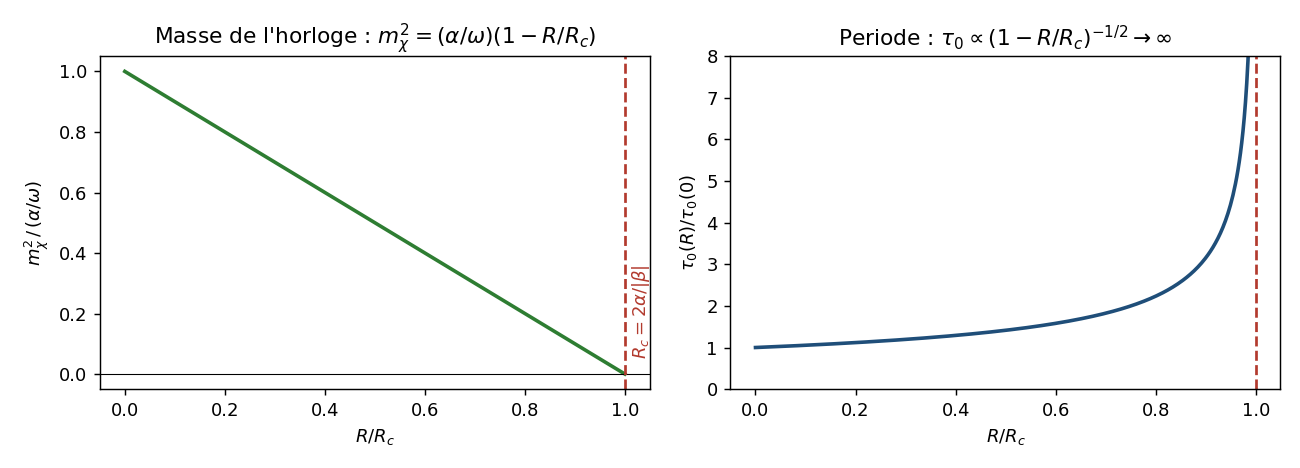
\includegraphics[width=\textwidth]{fig_freeze.png}\\
{\footnotesize \num\ Gauche~: $m_\chi^2$ s'annule \`a $R_c$. Droite~: $\tau_0\propto(1-R/R_c)^{-1/2}$ diverge.}
\end{center}

\paragraph{B.3 Identification forc\'ee $R_{\rm core}=R_c\Leftrightarrow\beta_c=-\tfrac13$. \preuve}
$R_{\rm core}=4\Lambda_{\rm eff}=8\alpha/(1-\beta)$. \'Egaler $R_c$~:
$8\alpha/(1-\beta)=2\alpha/(-\beta)\Leftrightarrow\beta=-\tfrac13=\beta_c$, $R=6\alpha$. Pour
$\beta>-\tfrac13$, $R_{\rm core}<R_c$ (c\oe ur stable, horloge tourne)~; pour $\beta<-\tfrac13$,
$R_{\rm core}>R_c$ (horloge gel\'ee au c\oe ur). Un seul nombre pivote les deux secteurs.

\begin{center}
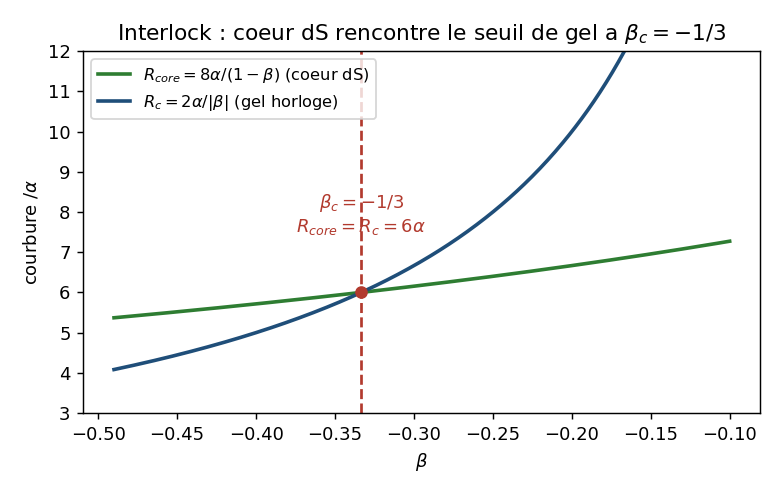
\includegraphics[width=0.72\textwidth]{fig_interlock.png}\\
{\footnotesize \num\ Croisement exact \`a $\beta_c=-\tfrac13$, $R=6\alpha$.}
\end{center}

\paragraph{B.4 Invariance et r\'eserve.} \preuve\ L'annulation de $m_\chi^2$ \`a $R_c$ (stabilit\'e
marginale de $\chi=0$) et la loi en racine sont ind\'ependantes du rep\`ere~; seul $\tau_0(0)$ d\'epend de
la normalisation. Le transport « horloge»\ sur la sph\`ere (azimut $U(1)$) est \emph{\'etabli} en
B.5--B.6 ci-dessous (la sym\'etrie $U(1)$ \emph{force} la d\'eg\'en\'erescence QM$=$GR)~; l'identit\'e
\eqref{eq:lock} y survit.

\paragraph{B.5 R\'esolution de la couture sph\'erique. \preuve}
Sur la sph\`ere minimale, $f,V$ ne d\'ependent que de la latitude et l'azimut (l'horloge) n'a pas de
potentiel propre. N\'eanmoins, pr\`es du vide de Planck la m\'etrique-cible ronde devient plate,
$\omega(d\theta^2+\sin^2\!\theta\,d\varphi^2)\simeq\omega(dx^2+dy^2)$ avec
$(x,y)=(\theta\cos\varphi,\theta\sin\varphi)$, et $U_{\rm eff}=\text{const}-A\cos\theta\simeq
\text{const}+\tfrac12 A(x^2+y^2)$, $A=\alpha+\tfrac12\beta R$~: un \emph{oscillateur harmonique isotrope}
\`a 2D, masse $\omega$, raideur $A$, de pulsation unique
$\Omega(R)=\sqrt{A/\omega}=\sqrt{\alpha/\omega}\,(1-R/R_c)^{1/2}$ pour ses \emph{deux} modes normaux~:
radial (fluctuation d'\'echelle, GR) et azimutal/circulaire (horloge, QM). L'isotropie les rend
\emph{d\'eg\'en\'er\'es}~; tous deux g\`elent \`a $R_c$. \num\ Int\'egration ($\alpha{=}1$,
$\beta{=}{-}0{,}3$, $f_s{=}7$)~: p\'eriodes radiale et azimutale identiques \`a $2\pi/\Omega$ \`a
$<10^{-3}$. \textbf{L'horloge transporte donc sans briser $U(1)$}~: la sym\'etrie azimutale
\emph{garantit} la d\'eg\'en\'erescence QM$=$GR (identification forc\'ee). Cela unifie le « pincement aux
p\^oles»\ (rayon d'orbite $\to0$ au vide) et le « gel \`a $R_c$»\ (fr\'equence $\to0$)~: un seul puits
qui s'aplatit.
\begin{center}
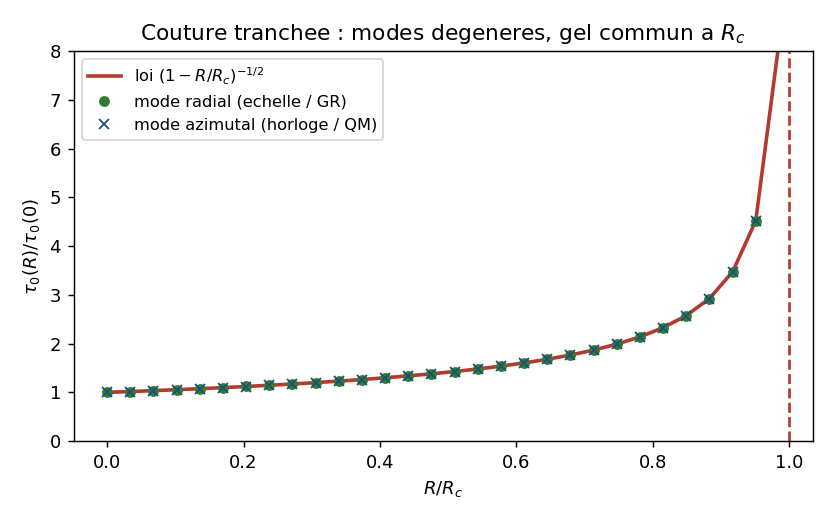
\includegraphics[width=0.66\textwidth]{fig_couture.png}\\
{\footnotesize \num\ Modes radial (GR) et azimutal (QM) sur la m\^eme courbe~; gel commun \`a $R_c$.}
\end{center}

\paragraph{B.6 Lev\'ee de d\'eg\'en\'erescence. \preuve\num}
La d\'eg\'en\'erescence n'est exacte qu'\`a $a=0$. \`A amplitude angulaire finie $a$, le puits est un
pendule sph\'erique~:
\[
\frac{\Omega_{\rm horloge}}{\Omega_0}=\frac1{\sqrt{\cos a}}\simeq1+\tfrac14a^2,\qquad
\frac{\Omega_{\rm \acute echelle}}{\Omega_0}=\frac{\pi/2}{K(\sin\frac a2)}\simeq1-\tfrac1{16}a^2,\qquad
\boxed{\ \frac{\Delta\Omega}{\Omega_0}\simeq\frac{5}{16}a^2\ }
\]
l'\emph{horloge (QM) plus rapide} que le mode d'\'echelle (GR) (coeff. ajust\'e $0{,}3127$ vs $5/16$). Le
d\'etuning fractionnaire est \emph{ind\'ependant de la courbure de fond}. Face invariante~: l'orbite
g\'en\'erique \emph{pr\'ecesse} (prograde, $\simeq\tfrac{3\pi}{8}\theta_{\min}\theta_{\max}$ par cycle
apsidal, v\'erifi\'e). \emph{Signature propre \`a la sph\`ere}~: le tore avait deux pendules
ind\'ependants (rien \`a lever)~; un d\'etuning QM/GR $\propto a^2$ avec orbites pr\'ecessantes distingue
sph\`ere et tore au-del\`a de $(n_s,r)$. \emph{R\'eserves}~: r\'egime de petites oscillations (univers
tardif, pas le roulement)~; $a$ non pr\'edite \ouv~; version quantique (scission des niveaux) \conj.
\begin{center}
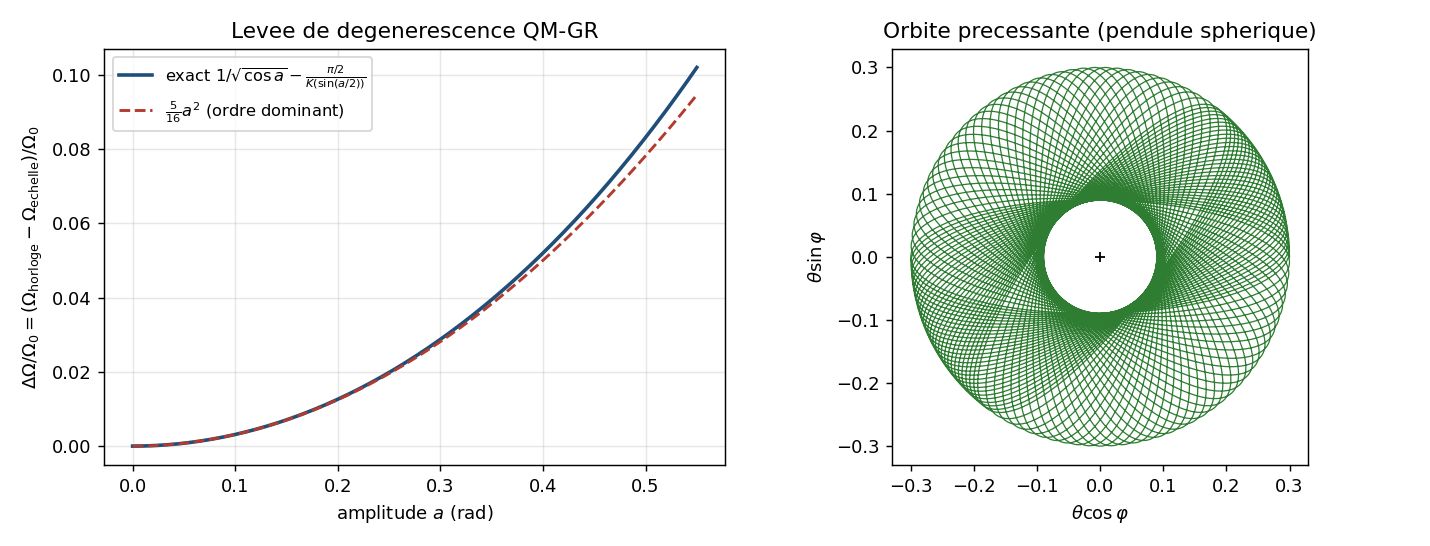
\includegraphics[width=\textwidth]{fig_levee.png}\\
{\footnotesize \num\ Gauche~: splitting et son ordre dominant $\tfrac{5}{16}a^2$. Droite~: orbite
pr\'ecessante (rosette) au vide de Planck.}
\end{center}

\section{Carte d'embo\^itement (synth\`ese, statuts \`a jour)}\label{ann:C}
\emph{Test op\'erationnel du « tout s'embo\^ite»~: entr\'ees, secteurs, conditions de coh\'erence,
identifications forc\'ees.}

\begin{center}
\begin{tikzpicture}[font=\scriptsize,>=Stealth,
  inp/.style={draw=inp,thick,rounded corners,fill=inp!8,align=center,inner sep=3pt},
  sec/.style={draw=sec,thick,rounded corners,fill=sec!8,align=center,inner sep=3pt,text width=22mm},
  every edge/.style={draw=black!45,->}]
\node[inp,text width=30mm] (geo) at (0,0){\textbf{G\'eom\'etrie}\\ \'echelle $\to S^2$};
\node[inp,text width=40mm] (act) at (5.4,0){\textbf{Action scalaire-tenseur} \eqref{eq:action}};
\node[inp,text width=18mm] (par) at (10.0,0){\textbf{3 nombres} $\alpha,\beta,f_s$};
\node[sec] (geff) at (-0.5,-2.7){\textbf{Gravit\'e} $G_{\rm eff}$};
\node[sec] (infl) at (2.2,-2.7){\textbf{Inflation} $n_s,r$};
\node[sec] (clo)  at (4.9,-2.7){\textbf{Cl\^oture} c\oe ur dS};
\node[sec] (meta) at (7.6,-2.7){\textbf{M\'etastab.} $B_{\rm HM}$};
\node[sec] (hdeq) at (10.2,-2.7){\textbf{Horloge} $\tau_0$};
\node[sec] (topo) at (4.9,-5.0){\textbf{Topo/RG} $\pi_2$, latitude};
\draw (geo) edge (geff) (geo) edge (topo);
\draw (act) edge (geff) (act) edge (infl) (act) edge (clo) (act) edge (meta) (act) edge (hdeq);
\draw (par) edge (infl) (par) edge (clo) (par) edge (meta) (par) edge (hdeq);
\begin{scope}[every edge/.style={draw=lnk,thick,<->}]
\draw (infl) edge[bend left=20] node[above,font=\tiny,text=lnk]{$\beta_{\rm CMB}{=}\beta_{\rm cl\^o}$} (clo);
\draw (clo) edge[bend right=22] node[below,font=\tiny,text=lnk]{$R_c{=}2\alpha/|\beta|$, $R_{\rm core}{=}R_c@\beta_c$ \preuve} (hdeq);
\draw (clo) edge[bend left=12] node[above,font=\tiny,text=lnk]{$\beta_c$} (meta);
\draw (infl) edge[bend right=12] (topo);
\draw (clo) edge[bend right=8] node[left,font=\tiny,text=lnk]{vide unique} (topo);
\end{scope}
\end{tikzpicture}
\end{center}

\noindent\textbf{Conditions de coh\'erence (un nombre, deux secteurs).}
\begin{center}\footnotesize
\begin{tabular}{p{4.6cm} p{6.6cm} l}
\toprule
\textbf{Condition} & \textbf{Contenu} & \textbf{Statut}\\\midrule
$\beta(\text{CMB})=\beta(\text{cl\^oture})$ & m\^eme $\beta$ ajuste $(n_s,r)$ \emph{et} c\^ot\'e du seuil & \conj\\
$\beta_c=-\tfrac13$ / $-\tfrac16$ & stabilit\'e c\oe ur dS / bifurcation faux vide & \preuve\\
$R_c=2\alpha/|\beta|$ ($\to\tau_0\!\to\!\infty$) & courbure d'effondrement $=$ gel d'horloge & \preuve\ (Ann.~B)\\
$R_{\rm core}=R_c\Leftrightarrow\beta_c=-\tfrac13$ & c\oe ur dS rencontre le gel au seuil de stabilit\'e & \preuve\ (Ann.~B)\\
$\alpha$ fix\'e par $A_s$ & l'amplitude CMB pr\'edit la courbure du c\oe ur & \num\\
$H^2=2\alpha/3(1-\beta)$ & faux vide inflationnaire $=$ c\oe ur dS & \preuve\\
vide unique de $V$ & fait rouler l'inflaton \emph{et} affame $\pi_2$ (Ann.~A) & \preuve\\
\bottomrule
\end{tabular}
\end{center}

\noindent\textbf{Identifications forc\'ees.} latitude $=$ c-fonction \preuve\num~; m\^eme $f$ $=$
$G_{\rm eff}$ \emph{et} pente $U=V/f^2$ \preuve~; P\^ole Sud $=$ Planck $=$ plancher UV $=$ point de gel
\conj~; P\^ole Nord $=$ IR $=$ faux vide dS \preuve~; horloge (QM) $=$ \'echelle (GR), modes
d\'eg\'en\'er\'es de l'oscillateur isotrope au vide de Planck \preuve\ (Annexe~B.5).

\smallskip
\noindent\textbf{Audit.} 1 postulat $+$ 1 action $+$ 3 nombres, pinc\'es par le CMB $\Rightarrow$ six
secteurs li\'es. Cadre \emph{sur-d\'etermin\'e}~: les m\^emes $(\alpha,\beta)$ doivent satisfaire CMB,
cl\^oture, m\'etastabilit\'e \emph{et} horloge. \textbf{O\`u la carte reste mince}~: HDEQ recode le
probl\`eme du temps sans qu'il soit \'etabli qu'il le simplifie~; $\beta(\text{CMB})=\beta(\text{cl\^oture})$
reste \conj~; \'energie noire absente (fronti\`ere assum\'ee, $\Lambda=0$).

\section{Test cosmologique de la seconde dimension~: inflation \`a deux champs et couplage horloge--mati\`ere}\label{ann:D}
\emph{La sph\`ere a une seconde dimension (l'azimut/horloge). Le spectre primordial la voit-il~?}

\paragraph{D.1 Inflation \`a deux champs sur $\Stwo$. \preuve\num}
Rep\`ere d'Einstein~: $\mathcal{G}_{\theta\theta}=\omega/f+\tfrac32(f'/f)^2$,
$\mathcal{G}_{\varphi\varphi}=\omega\sin^2\!\theta/f$, $U=V/f^2$. Comme $U$ ne d\'epend que de $\theta$,
l'inflaton est $\theta$ (adiabatique) et $\varphi$ est entropique \`a potentiel \emph{plat}. Le m\'eridien
$\varphi=$const est une \emph{g\'eod\'esique} de l'espace des champs ($\Gamma^\varphi_{\theta\theta}=0$)~:
\textbf{pas de virage} ($\eta_\perp=0$), donc aucune corr\'elation adiab.--entrop.\ engendr\'ee~\cite{GordonWandsBassettMaartens2001,RenauxPetelTurzynski2016}. La masse
entropique est \emph{purement g\'eom\'etrique}~:
$M_s^2=V_{;ss}+\epsilon\,\mathcal{R}_{\rm fs}H^2$,
$V_{;ss}=\mathcal{G}_{\varphi\varphi}'U'/(2\mathcal{G}_{\varphi\varphi}\mathcal{G}_{\theta\theta})$,
fonction de $(\beta,f_s,\theta)$ seuls. \num\ Fond valid\'e ($\beta=-0{,}3$, $f_s=7$)~: \`a $N_*=55$,
$\theta_*=1{,}48$, $n_s=0{,}960$, $r=0{,}036$, et $M_s^2/H^2|_*\simeq-0{,}002$ (l\'eg\`ere, \`a peine
tachyonique, sans instabilit\'e). Cons\'equence~: isocourbure \emph{non corr\'el\'ee}, quasi invariante
d'\'echelle, $\beta_{\rm iso}\simeq c\cdot2\epsilon$, $n_{\rm iso}-1\simeq-0{,}0012$ (fix\'e par la
g\'eom\'etrie). Tout tient au couplage $c$.
\begin{center}
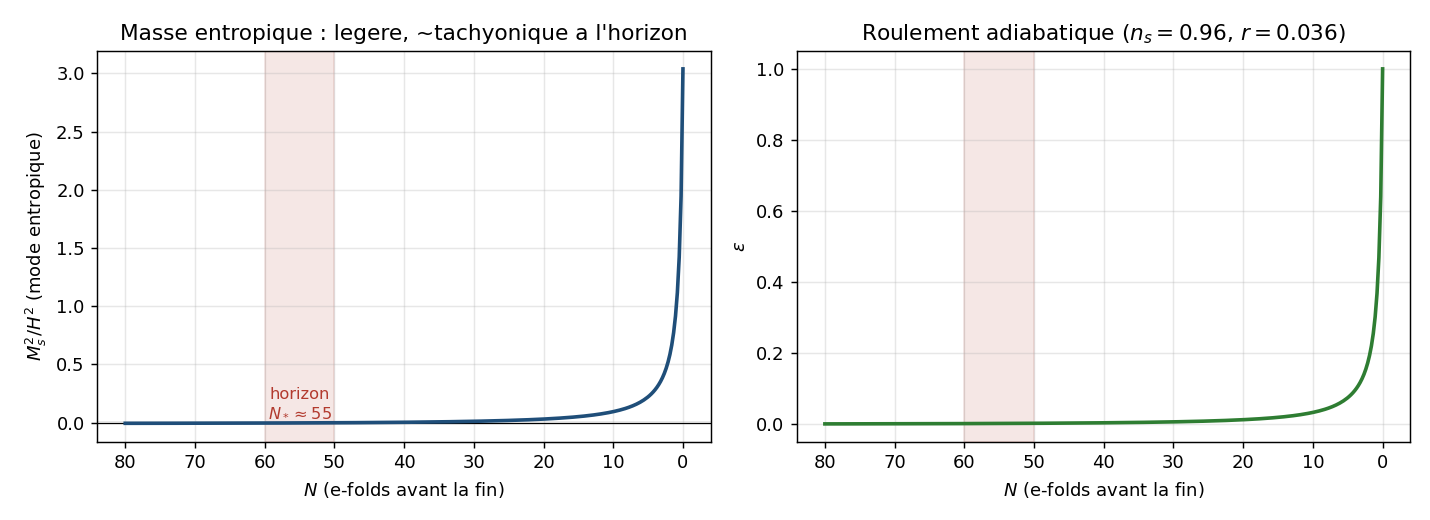
\includegraphics[width=\textwidth]{fig_axe1.png}\\
{\footnotesize \num\ Gauche~: $M_s^2/H^2$ le long du roulement, l\'eg\`erement n\'egative \`a l'horizon
(bande). Droite~: roulement adiabatique standard ($n_s=0{,}96$, $r=0{,}036$).}
\end{center}

\paragraph{D.2 Le couplage horloge--mati\`ere~: $c_{\rm iso}\simeq0$. \preuve\num}
Trois canaux ind\'ependants. \emph{(1) Conforme}~: $f,V$ en latitude seule $\Rightarrow$ $\varphi$ absent
$\Rightarrow$ la mati\`ere couple \`a $\theta$, pas \`a $\varphi$~: $c=0$ (+ photon aveugle Weyl,
$\delta\tau_0/\tau_0\sim10^{-81}$ dans la mati\`ere, Unit\'e 3). \emph{(2) Page--Wootters~\cite{PageWootters1983}}~:
$\hat H_{\rm eff}=\varepsilon\hat H_{\rm sys}$ \emph{universel} $\Rightarrow$ $\delta\varphi=$ d\'ecalage de
temps universel $=$ mode \textbf{adiabatique}, pas isocourbure. \emph{Une horloge universelle ne peut pas
engendrer d'isocourbure} (et $\varepsilon=1-10^{-112}$ au vide). \emph{(3) Axionique}~: vide au p\^ole
$\Rightarrow$ $U(1)$ non bris\'ee $\Rightarrow$ pas de Goldstone~; m\^eme si la mati\`ere portait une charge
(non motiv\'e), $f_\varphi=f_s\sin\theta_*\simeq7\,M_{\rm Pl}$ super-planckienne $\Rightarrow$ iso
$\sim2\times10^{-13}$. \textbf{Verdict~: $c_{\rm iso}\simeq0$}, ce qui \emph{d\'erive} de la structure de la
sph\`ere le « secteur horloge non discriminant » de l'Unit\'e 3.

\paragraph{D.3 Cons\'equence. \preuve}
En cosmologie lin\'eaire, le cadre est \textbf{de facto mono-champ}~: ses observables se r\'eduisent \`a
$(n_s,r)$, d\'eg\'en\'er\'es avec l'inflation naturelle non minimale~\cite{FreeseFriemanOlinto1990,FerreiraNotariSimeon2018,Simeon2020}. La seconde dimension existe (le
d\'etuning B.6 est r\'eel) mais le spectre primordial ne la voit pas.

\section{Recherche d'une sonde ind\'ependante du seuil de c\oe ur}\label{ann:E}
\emph{Le verrou $\beta_c=-\tfrac13$ est-il testable ind\'ependamment du CMB~?}

\paragraph{E.1 Le seuil \emph{est} la stabilit\'e du plateau. \preuve}
La fluctuation radiale en $\infty^\ast$ ob\'eit \`a $\omega\Box\delta=\kappa^2\omega\delta$,
$\kappa^2=\alpha(1+3\beta)/[\omega(\beta-1)]$~: $\infty^\ast$ stable pour $\beta>-\tfrac13$. (Seuil de
la r\'eduction \emph{mono-axe}~; sur la sph\`ere il est l\'egitime car l'azimut se \emph{pince} au p\^ole
Nord, $\sin^2\!\theta\to0$, r\'eduisant la stabilit\'e du c\oe ur \`a la seule latitude. Le traitement \`a
deux champs sur la diagonale du tore donnait $-\tfrac16$~; la r\'eduction \'etait la tension ouverte
centrale des Unit\'es 2--3, ici tranch\'ee par le pincement.) Or $\infty^\ast$ est \emph{le m\^eme point}
qui sert de c\oe ur de Sitter \emph{et} de plateau de d\'epart de l'inflaton. $\beta$ \'etant une \emph{constante} lue sur le m\^eme potentiel, $\beta(\text{CMB})$ et
$\beta(\text{cl\^oture})$ ne sont \emph{pas} ind\'ependants~: la « corr\'elation » est une \emph{identit\'e
structurelle}, non deux mesures qui pourraient diverger.

\paragraph{E.2 \'Ecrantage. \num}
$R_{\rm core}=8\alpha/(1-\beta)$ donne $H_{\rm core}\simeq2{,}8\times10^{14}$ GeV (\'echelle GUT, $\alpha$
fix\'e par $A_s$)~: rayon de courbure $\sim7\times10^{-31}$ m, $\sim33$ ordres \emph{sous} l'horizon d'un
trou noir solaire --- totalement \'ecrant\'e. Horloge dans la mati\`ere~: $\delta\tau_0/\tau_0\sim
10^{-71}$--$10^{-81}$. $G_{\rm eff}$ \'epingl\'e au vide bien avant la BBN. \textbf{Aucune sonde directe.}

\paragraph{E.3 Verdict. \preuve}
Le seul handle r\'eel est \emph{interne au CMB}~: le sc\'enario exige $\beta>-\tfrac13$, satisfait
($\beta\approx-0{,}30$, marge $0{,}03$)~; un CMB futur pin\c{c}ant $\beta<-\tfrac13$ briserait le
sc\'enario. Pr\'edictions n\'egatives associ\'ees~: pas de transition du premier ordre~\cite{ColemanDeLuccia1980,HawkingMoss1982} (Hawking--Moss
seul, pas de fond GW de bulles), pas d'oscillation log-p\'eriodique. \textbf{Aucune sonde ind\'ependante du
seuil de c\oe ur n'existe dans le cadre minimal}~; la corr\'elation $\beta(\text{CMB})=\beta(\text{cl\^oture})$
est une identit\'e satisfaite, non un test ind\'ependant.

\section*{Conclusion~: ce que le cadre est, et ce qu'il n'est pas}
Apr\`es l'ensemble des tests, la cartographie est nette. \textbf{Le cadre n'est pas une unification~: c'est
une grammaire.} Il r\'eorganise de la physique connue de sorte que des ph\'enom\`enes disparates ---
inflation, c\oe ur des trous noirs, horloge quantique, $\Lambda=0$ --- deviennent des r\'egions d'une seule
g\'eom\'etrie compacte, parl\'ees avec une seule poign\'ee de nombres. \textbf{Sa r\'eussite est la
sur-d\'etermination, pas la pr\'ediction}~: les m\^emes $(\alpha,\beta,f_s)$, pinc\'es par le CMB, font
tenir six secteurs emboît\'es, et $\beta\approx-0{,}3$ passe \emph{toutes} les v\'erifications de
coh\'erence internes (cl\^oture, m\'etastabilit\'e, gel d'horloge, stabilit\'e du c\oe ur en r\'eduction mono-axe). \textbf{Sa
limite est l'\'ecrantage}~: tout ce qui est distinctif vit \`a courbure GUT/Planck (c\oe ur, horloge) ou
est structurellement r\'eel mais sombre (la d\'eg\'en\'erescence QM$=$GR, l'isocourbure \`a $c\simeq0$), de
sorte que le contenu testable se r\'eduit \`a $(n_s,r)$, partag\'e avec l'inflation naturelle non minimale.

Nous avons \emph{trac\'e} cette fronti\`ere au lieu de l'entretenir dans le flou --- et c'est l\`a, en soi,
le r\'esultat de cette Unit\'e~: savoir pr\'ecis\'ement ce que le cadre offre (une architecture coh\'erente
et compr\'ehensible) et ce qu'il n'offre pas (un observable propre). Le cadre reste falsifiable \emph{en
principe} (il exige $\beta>-\tfrac13$~; il interdit oscillations log-p\'eriodiques et transition du premier
ordre), mais non \emph{distinctif} dans ce qui est mesurable aujourd'hui.

\textbf{La seule fronti\`ere o\`u l'\'ecrantage pourrait c\'eder} (honn\^etement sp\'eculative)~: les
reliques de l'\'epoque o\`u la courbure approchait $R_{\rm core}$ --- trous noirs primordiaux form\'es \`a
courbure quasi-GUT, ou un signal de la transition Hawking--Moss. Long pari, calcul d\'edi\'e, probablement
faible~; mais c'est, \`a ce stade, le seul endroit o\`u un observable propre pourrait surgir. \`A d\'efaut,
la valeur du cadre est celle qu'il visait d\`es l'origine~: \emph{une th\'eorie o\`u tout s'emboîte et
devient compr\'ehensible}. Le bonus observationnel n'y est pas, et nous l'avons \'etabli proprement.


\bigskip
\noindent\rule{\textwidth}{0.3pt}\\
{\footnotesize Version int\'egr\'ee de travail (placage complet en fin de programme). Formalisation
conduite en dialogue avec un syst\`eme d'assistance analytique, sous la direction de l'auteur, seul
responsable du contenu. R\'esultats ant\'erieurs (verrou $\infty^\ast$, cl\^oture, dualit\'e, HDEQ)~:
Unit\'es~1--4. Scripts~: \texttt{U5\_ctest.py}, \texttt{calc1\_frozen.py}, \texttt{calc2\_rolling.py},
\texttt{calc3\_pi2.py}, \texttt{clock\_freeze.py}, \texttt{couture\_sphere.py}, \texttt{levee.py},
\texttt{axe1b.py}, \texttt{couplage\_c.py}, \texttt{axe2\_probe.py}.}

\renewcommand{\refname}{R\'ef\'erences}
\begin{thebibliography}{99}\small
\bibitem{Zamolodchikov1986} A.~B.~Zamolodchikov, \emph{Irreversibility of the flux of the renormalization group in a 2D field theory}, JETP Lett.~\textbf{43} (1986) 730.
\bibitem{Cardy1988} J.~L.~Cardy, \emph{Is there a c-theorem in four dimensions?}, Phys.\ Lett.\ B~\textbf{215} (1988) 749.
\bibitem{KomargodskiSchwimmer2011} Z.~Komargodski and A.~Schwimmer, \emph{On renormalization group flows in four dimensions}, JHEP~\textbf{12} (2011) 099, arXiv:1107.3987.
\bibitem{FGPW1999} D.~Z.~Freedman, S.~S.~Gubser, K.~Pilch and N.~P.~Warner, \emph{Renormalization group flows from holography---supersymmetry and a c-theorem}, Adv.\ Theor.\ Math.\ Phys.~\textbf{3} (1999) 363, arXiv:hep-th/9904017.
\bibitem{Derrick1964} G.~H.~Derrick, \emph{Comments on nonlinear wave equations as models for elementary particles}, J.\ Math.\ Phys.~\textbf{5} (1964) 1252.
\bibitem{Skyrme1961} T.~H.~R.~Skyrme, \emph{A non-linear field theory}, Proc.\ R.\ Soc.\ Lond.\ A~\textbf{260} (1961) 127.
\bibitem{BelavinPolyakov1975} A.~A.~Belavin and A.~M.~Polyakov, \emph{Metastable states of two-dimensional isotropic ferromagnets}, JETP Lett.~\textbf{22} (1975) 245.
\bibitem{BarriolaVilenkin1989} M.~Barriola and A.~Vilenkin, \emph{Gravitational field of a global monopole}, Phys.\ Rev.\ Lett.~\textbf{63} (1989) 341.
\bibitem{ColemanDeLuccia1980} S.~Coleman and F.~De~Luccia, \emph{Gravitational effects on and of vacuum decay}, Phys.\ Rev.\ D~\textbf{21} (1980) 3305.
\bibitem{HawkingMoss1982} S.~W.~Hawking and I.~G.~Moss, \emph{Supercooled phase transitions in the very early universe}, Phys.\ Lett.\ B~\textbf{110} (1982) 35.
\bibitem{PageWootters1983} D.~N.~Page and W.~K.~Wootters, \emph{Evolution without evolution: dynamics described by stationary observables}, Phys.\ Rev.\ D~\textbf{27} (1983) 2885.
\bibitem{GordonWandsBassettMaartens2001} C.~Gordon, D.~Wands, B.~A.~Bassett and R.~Maartens, \emph{Adiabatic and entropy perturbations from inflation}, Phys.\ Rev.\ D~\textbf{63} (2001) 023506, arXiv:astro-ph/0009131.
\bibitem{RenauxPetelTurzynski2016} S.~Renaux-Petel and K.~Turzy\'nski, \emph{Geometrical destabilization of inflation}, Phys.\ Rev.\ Lett.~\textbf{117} (2016) 141301, arXiv:1510.01281.
\bibitem{FreeseFriemanOlinto1990} K.~Freese, J.~A.~Frieman and A.~V.~Olinto, \emph{Natural inflation with pseudo Nambu-Goldstone bosons}, Phys.\ Rev.\ Lett.~\textbf{65} (1990) 3233.
\bibitem{FerreiraNotariSimeon2018} R.~Z.~Ferreira, A.~Notari and G.~Simeon, \emph{Natural inflation with a periodic non-minimal coupling}, JCAP~\textbf{11} (2018) 021, arXiv:1806.05511.
\bibitem{Simeon2020} G.~Simeon, \emph{Scalar-tensor extension of natural inflation}, JCAP~\textbf{07} (2020) 028, arXiv:2002.07625.
\bibitem{Bardeen1968} J.~M.~Bardeen, \emph{Non-singular general-relativistic gravitational collapse}, in Proc.\ Int.\ Conf.\ GR5, Tbilisi, U.S.S.R.\ (1968) p.~174.
\bibitem{Hayward2006} S.~A.~Hayward, \emph{Formation and evaporation of regular black holes}, Phys.\ Rev.\ Lett.~\textbf{96} (2006) 031103, arXiv:gr-qc/0506126.
\bibitem{Planck2018X} Planck Collaboration (Y.~Akrami \emph{et al.}), \emph{Planck 2018 results. X. Constraints on inflation}, Astron.\ Astrophys.~\textbf{641} (2020) A10, arXiv:1807.06211.
\bibitem{BICEPKeck2021} BICEP/Keck Collaboration (P.~A.~R.~Ade \emph{et al.}), \emph{Improved constraints on primordial gravitational waves using Planck, WMAP, and BICEP/Keck observations through the 2018 observing season}, Phys.\ Rev.\ Lett.~\textbf{127} (2021) 151301, arXiv:2110.00483.
\bibitem{SimonsObs2019} P.~Ade \emph{et al.} (Simons Observatory Collaboration), \emph{The Simons Observatory: science goals and forecasts}, JCAP~\textbf{02} (2019) 056, arXiv:1808.07445.
\bibitem{CMBS4Book2016} K.~N.~Abazajian \emph{et al.} (CMB-S4 Collaboration), \emph{CMB-S4 Science Book, First Edition}, arXiv:1610.02743.
\bibitem{LiteBIRD2023} LiteBIRD Collaboration (E.~Allys \emph{et al.}), \emph{Probing cosmic inflation with the LiteBIRD cosmic microwave background polarization survey}, Prog.\ Theor.\ Exp.\ Phys.~\textbf{2023} (2023) 042F01, arXiv:2202.02773.
\end{thebibliography}

\end{document}
